%Kan i vissa fall delas upp i metodbeskrivning, experimentell uppställning och arbetsgång. Att redogöra för sin metod är viktigt bland annat för att förklara varför den valda metoden ger ett tillförlitligt resultat. Alla antaganden och förenklingar måste anges och motiveras. Definiera matematiska modeller så att andra ingenjörer och forskare kan förstå vad du gjort.
%Exempelvis utnyttjades Microsoft Excel 2013 för att analysera mätresultaten och plotta mätdata.

% Här beskrivs metoden, ofta är det lämpligt att dela upp texten i ett antal underrubriker.
% Använd alltid högst tre rubrik-nivåer.

\begin{figure} [H]
\begin{center}
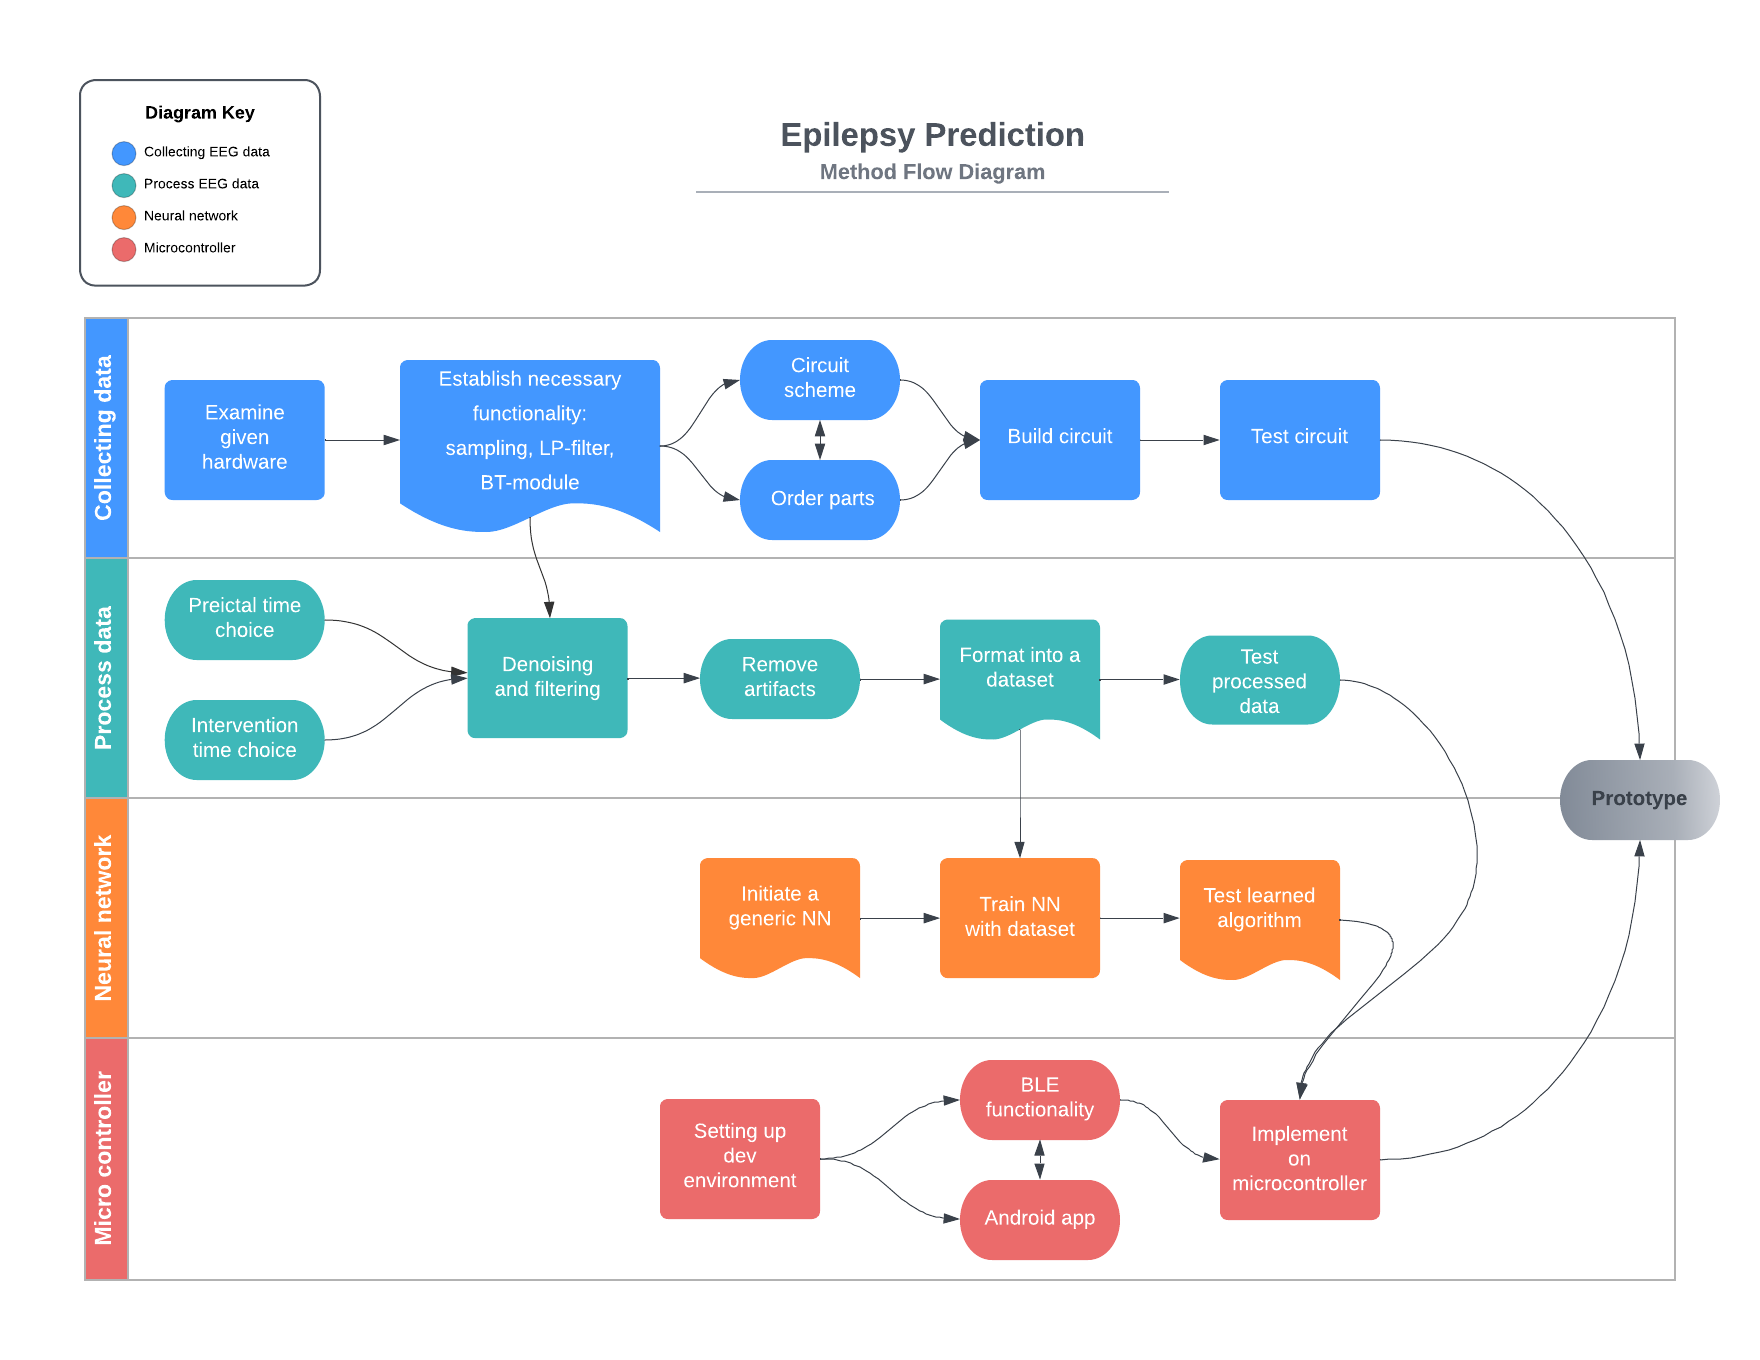
\includegraphics[width=0.7\textheight]{images/Epilepsy Prediction, method flow chart.png}
   \caption{A flow diagram depicting individual steps for the project as a whole.}
    \label{fig:flowmethod}
\end{center}
\end{figure}

For clarity, the project is divided into X parts, starting with the low-level hardware implementation and ending with the proposed classification methods.

\subsection{Hardware architecture}
The general structure of the hardware back-end of the project can be seen in \ref{fig:hw_struct}
\begin{figure} [H]
\begin{center}
\includesvg[inkscapelatex=false,width=\textwidth]{images/hw_struct2}
   \caption{Structure of the developed hardware design.}
    \label{fig:hw_struct}
\end{center}
\end{figure}

\subsubsection{Electrodes and filtering}
The semi-dry electrodes can be modeled as in figure(\ref{fig:Electrodes}) from \cite{electrodmodel}. Since the electrodes are sensitive to picking up noise from movements and the environment, it is essential to filter out the noise before it propagates in the system. It is achieved by placing an RC filter on the input. The filter is designed to have as low an R value as possible to mitigate the thermal noise and a value of C to set the cutoff frequency. This filter mainly reduces high-frequency noise, such as radio and cellphone signals. Figure (\ref{fig:Electrodes}) shows that the electrode model put a resistor in series with the RC filter that will affect the cutoff frequency. By simulating extreme values, the values on R and C can be chosen so the cutoff frequency remains inside the desired band of frequencies. Also, since the electrodes are sensitive to picking up surges when touched, an ESD protection IC circuit is added to the input of each electrode to protect against this. As mentioned, the thermal noise from the contact resistance can be a dominant factor. For example, the noise from the OP amps in the amplifier is $\SI{7.5}{\nano\volt/\sqrt{\hertz}}$, and thermal noise can be calculated as
\begin{equation}
    V_{Tnoise}=\sqrt{4*k_B*T*R}
\end{equation}
Where $k_B$ is Boltzmann's constant, T is the temperature in Kelvin and R the resistance in Ohm. So, for example, a contact resistance of $\SI{5000}{\ohm}$ gives a value of $\SI{9}{\nano\volt/\sqrt{\hertz}}$, but for a contact of 50000, it gives a value of $\SI{28}{\nano\volt/\sqrt{\hertz}}$. It is, therefore, essential to keep the contact between the electrode and scalp as good as possible. Otherwise, the contact noise would be dominant compared to the signal of interest.

The waveforms collected at the electrodes are generally in the $10-100$~{\textmu}V range, making them susceptible to noise from the outside and the rest of the circuitry. Also, the relevant signal amplitude needs to be increased to get as good performance as possible from the Adc. Due to this, the signals must be fed through an amplification step before any other conversions can be made. Another point important to consider is the electrode placement on the head, especially for the ground and reference electrode these are places according to the OpenBCI documentation \cite{OpenBCIcap} and can be seen in figure(\ref{fig:Electrodesplace}).
\begin{figure} [H]
\begin{center}
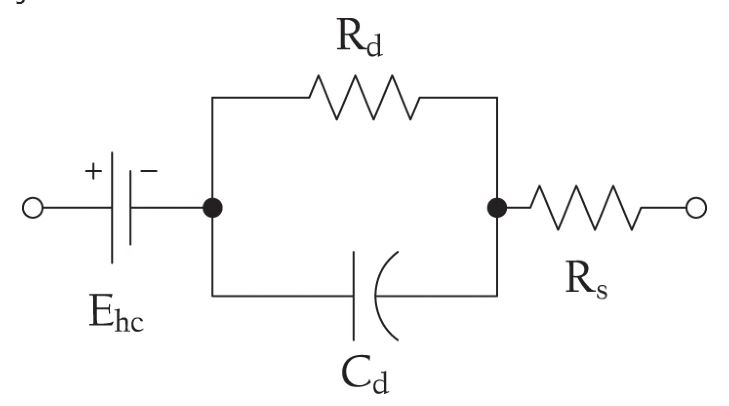
\includegraphics[scale=0.5]{images/electrodemodel.jpg}
   \caption{Model of scalp electrodes}
    \label{fig:Electrodes}
\end{center}
\end{figure}
\begin{figure} [H]
\begin{center}
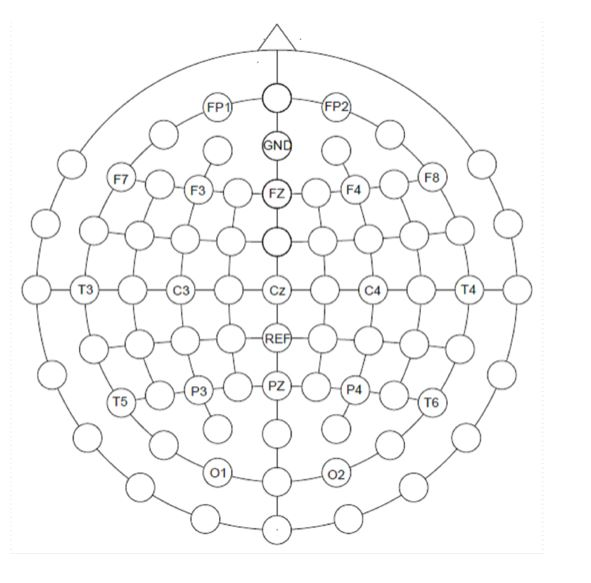
\includegraphics[scale=0.6]{images/Electrodeplacements.jpg}
   \caption{Description over electrode placements}
    \label{fig:Electrodesplace}
\end{center}
\end{figure}
\subsubsection{Amplification}
%Add IMAGE OF AMPLIFIER and Rail splitter
Due to the low signal levels and noise from the electrodes, amplification is needed to process the signals. The amplifier of choice is an instrumentation amplifier that utilizes differential amplification based on the design from \cite{EEamp}. Differential amplification works on the principle that the noise is equally coupled onto the terminals; therefore, only the wanted signal is amplified. An instrumentation amplifier has the advantage that the gain is easily changeable and has a high Common mode rejection ratio (CMRR). This high CMRR makes it the superior choice when dealing with EEG measurements. From figure(\ref{fig:amplifier}) the equation for the gain is set solely by varying $R_G
$, and the equation for the gain is given by
\begin{equation}
    A_d=(1+\dfrac{\SI{200}{\kilo\ohm}}{R_G})*A_{B}
\end{equation}
 Where $A_{B}$ is the gain from the buffer stage set by varying $R_{16}$ in figure(\ref{fig:amplifier}). This is to prevent the first stage from getting too close to the open loop gain of the OP amps but still being able to produce a large gain. Since the hardware is driven from a single battery, we cannot obtain voltages below ground on our output. It is solved with a rail splitter circuit, as seen in figure(\ref{fig:railsplit}). This circuit splits the battery voltage into two voltages, V+ and V-, and creates a new virtual ground reference. The chosen design uses readily available and affordable components it is easy to assemble and test. With these new rail voltages, it is possible to achieve outputs between these. If a DC offset on the output is wanted, this can be adjusted through the Vref terminal of the amplifier. It is connected to a buffered voltage divider where any value on Vref can be achieved with the appropriate choice of resistors.
\subsubsection{Anti-aliasing filter}
Before the ADC samples the signal, an anti-aliasing filter is needed to prevent the signal from getting corrupted. An aliasing filter with a cutoff frequency at half the Nyquist frequency is needed to avoid any signal aliasing. It is achieved by implementing a second-order Butterworth lowpass filter in the Sallen-Key topology. The Butterworth filter gives a steady amplitude response and has a suitable roll-off in the transition region of $\SI{-40}{\deci\bel}/decade$. 

\subsubsection{Analog-to-digital conversion}
\label{section:ADC}
Once the signals are collected and amplified, the MCU requires they be converted from the analog to the digital domain. 

Because of the nature of the waveform, a high signal-to-noise ratio and resolution was the priority in the selection of analog-to-digital converters. This ruled out the on-board ADCs provided as part of the MCU, and most of the ADCs available on the market. This, combined with the silicone shortage, led us to use higher precision, single-channel ADCs and multiplex between them. The final architecture consists of 16 single-channel analog to digital converters connected to two multiplexers. The MUX1 in \ref{fig:hw_struct} handles the converted, digital signals, and feeds them to the MCU. The design of the ADCs in question means there is a second signal, DRDYx in the figure, that is set high by the corresponding ADC once a sample is converted and ready to be sent. The DRDYx rising edge triggers an interrupt in the MCU, which collects the sample, and increments the ADC Select signal, which switches the multiplexers to the next ADC at which point the procedure is repeated. Once a sample has been received from each of the ADCs, the ADC Select signal wraps back to 0, and the preprocessing/classification procedure can be initiated.

\subsubsection{Microcontroller and communication}
After the analog-to-digital conversion is made, the data is ready for processing. The processing is done on an STM32L431RCT6 which is the microcontroller of use. A battery or USB drives it to an LDO voltage regulator to decrease the voltage to 3.3V. The PCB also can communicate over UART. The UART connection is connected via a digital isolator to isolate the ground and power to keep the noise levels down from, for example, ground loops. Programming of the microcontroller is carried out over SWD.

\subsubsection{User interface}
A BLUENRG-M0A low-energy Bluetooth module is implemented on the PCB. This enables the user to pair the device to an Android mobile device using a simple app developed as part of the project. Once a seizure is detected, a notification is sent to the mobile device allowing the user to prepare themselves for the attack.
The Bluetooth implementation leverages a single service, containing one single characteristic, which changes whenever the user is to be warned. The characteristic uses the notify property to push data to the client mobile phone.
The implementation is aided by the X-CUBE-BLE1 software pack provided by the module's vendor. It contains a hardware abstraction layer, which allowed for relatively easy implementation.

\subsubsection{Simulation}
The nature of the project implies that testing the system is not trivial. Setting up a clinical trial was simply not an option, so a simulation environment was created to at least partly verify the system's functionality.



The simulation environment functions upon the idea that part of the hardware design highlighted in figure \ref{fig:blackbox} can be treated as a black box relative to the rest of the system. This implies that it can be simulated, with the digital SPI signal being configurable.

\begin{figure} [H]
\begin{center}
\includesvg[inkscapelatex=false,width=\textwidth]{images/blackbox}
   \caption{From the MCU's frame of reference, the part of the system specified in this figure can be treated as a black box.}
    \label{fig:blackbox}
\end{center}
\end{figure}

This can be leveraged, as shown in figure \ref{fig:simulator}, to create a simulation environment where a PC feeds a NUCLEO development board with an arbitrary signal via USB, the NUCLEO board converts it to an SPI signal and feeds it to the MCU following the protocol specified in section \ref{section:ADC}. This ensures that from the frame of reference of the MCU, the simulator is indistinguishable from the data collection circuitry, which implies that the pre-processing and classification algorithms can be verified on-chip without changing any code, and most importantly without needing real-life clinical trials.

\begin{figure} [H]
\begin{center}
\includesvg[inkscapelatex=false,width=\textwidth]{images/simulator}
   \caption{The hardware design of the simulator}
    \label{fig:simulator}
\end{center}
\end{figure}

The specific use case of the simulation environment in this project involved sending freely available EEG data collected during a clinical trial with epileptic patients \cite{CHB-MIT} over the USB connection, and verifying that the system was behaving as expected.

\subsection{Preprocessing}
%For the signal preprocessing a mixture of literature studies and programming in Python (later C) was done. First the minimal intervention time window was chosen to be 2 minutes, meaning that the prototype should be able to at least predict a seizure 2 minutes before the actual onset. This was concluded to be a small enough window to be achievable for first trials and big enough that it would actually be useful as a prediction device. Then a pre-ictal time choice of 30 min was chosen based on the study done by Teixeira et al (2014, p. 324-336) where they found that a pre-ictal time of 30.47 min was the most applicable average value.
The processing of data between the hardware filtering and prediction algorithms. Consists of both software filter's and artifact removal.

\subsubsection{Digital filters}
A Cascaded Integrator Comb (CIC) filter was first written in Matlab with the algorithms depicted in Rick Lyons ``A Beginner's Guide To Cascaded Integrator-Comb (CIC) Filters" \cite{CICguide} and then translated into C. For a better passband gain a compensating finite impulse response (FIR) filter was also written. But since later in the project it was concluded that data could not be changed, and CIC is a decimating filter, both these C function's were removed. Instead a lowpass FIR filter was started but could not be finished in time.

\subsubsection{Artifact removal}
First a Notch filter was implemented in Matlab together with a EEG signal processing tool named ``EEG lab". With this add-on the data was also denoised and the worst data artifacts was removed. This tool was useful for easily viewing the data but was never implemented in the micro controller because of it's complexity. Artifacts was instead processed with the blind source algorithm ICA. The algorithm was first implemented with open-source libraries in Python. Here it became apparent that the algorithms for ICA was to heavy and slow for the size of the EEG data to be measured. Instead a FastICA algorithm by Aapo Huvärinen was used utilizing maximum entropy approximations of differential entropy. This approach creates fast and robust fixed-point algorithms for this type of independent  component analysis \cite{fastICA}. So with this faster ICA algorithm and some open-source matrix help function's, a library was written in C. From this library the major output is the W matrix which is the estimated un-mixing matrix. It is then necessary to do an analysis of these estimated components to be able to separate what is the desired signal and whats and artifact which was done due to both lack of time and a lack of experience in the neuroscience field.

\subsection{Dataset}
For training purposes the CHB-MIT dataset was used. This dataset was recorded at the Boston children hospital on $22$ patient of ages $1.5 - 19$. The dataset was published on the $9th$ of June $2010$. The dataset is split into $23$ cases (one for each patient except $2$ that were for the same patient) numbered as chb$1$ to chb$23$. A case contains between $9$ and $42$ files containing roughly $23$ EEG signal channels, whit a resolution of $16$-bit these were sampled at a rate of $256$ samples per second. The data has labelled the start and end of seizures. (https://physionet.org/content/chbmit/1.0.0/)


\subsection{Formatting the dataset}

\subsubsection{C++ program}

A simple C++ application was set up to format the dataset in an environment that had more precise control and would be faster at a low level than Python, in which most of the other code was written in.

The program has a graphical interface in which you can click on a button to run a hardcoded function that generates a dataset in a txt file.

That function follows the following loop:

%filename += ".edf";
%
%			datapointer->ImportEDF(filename);
%			datapointer->LoadLabels(filename);
%			datapointer->MakeWindows();
%			datapointer->SortDataset();
%			datapointer->RemoveJunk();
%			//if (a % 5 == 0) {
%			//	datapointer->BalanceDataset();
%			//}
%		}
%	}
%	datapointer->BalanceDataset();
%	datapointer->ExportData("data/output/chb01.txt");
%	datapointer->Cleanup();

\begin{itemize}
    \item Import EDF file and translate into readable variables. This website was of great use for this: \url{https://www.teuniz.net/edfbrowser/edf\%20format\%20description.html}.
    \item Label the data in chunks of 256 time steps (1 second), 0 for inter-ictal (more than 30 minutes before seizure), 1 for pre-ictal (less than 5 minutes before seizure), and 2 for ictal (seizure).
    \item Make data windows for the same intervals, grayscale images of size 23 x 256 pixels.
    \item Sort data windows into 3 groups depending on label.
    \item Remove junk data and repeat until wanted dataset size is achieved.
\end{itemize}

Then the dataset is balanced so that each group of data windows shrinks to fit the size of the smallest group. This is done by randomly discarding data windows. \\

Finally, the dataset is exported into a txt file in ascii format. It would be possible and much more efficient to use binary instead of ascii for this, but an ascii file is possible to read in applications such as notepad, making it easier to debug. \\

\begin{figure}[H]
    \centering
    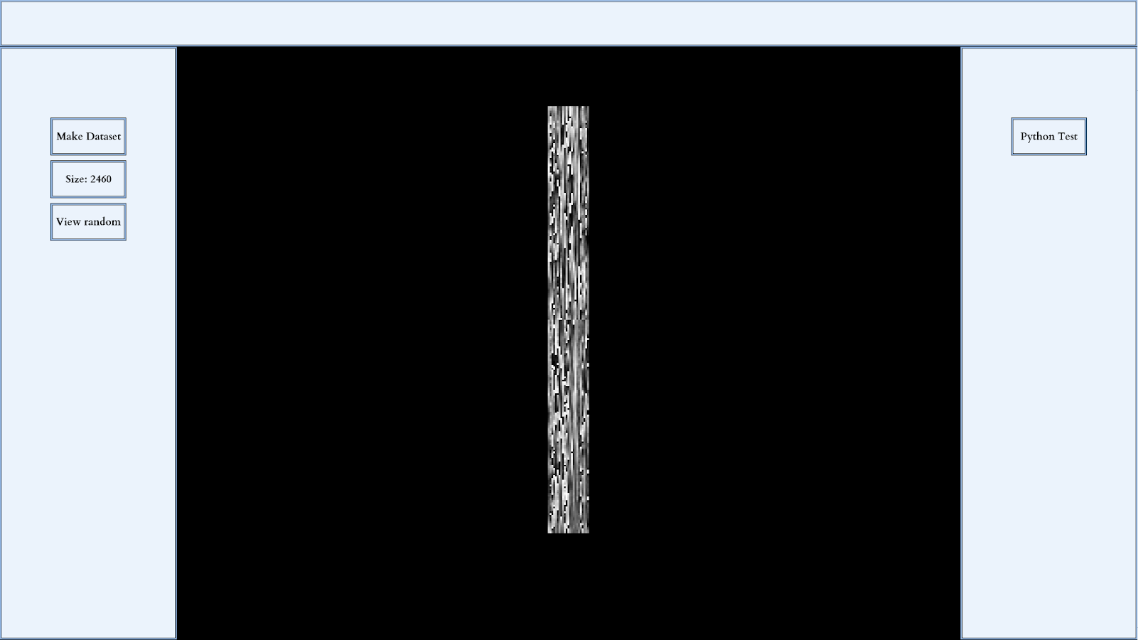
\includegraphics[width=1\textwidth]{images/datasetgenerator.PNG}
    \caption{The dataset generator has a simple visual interface that can be interacted with, as well as some feedback being given back to the user as the dataset is being generated.}
    \label{dataset_generator}
\end{figure}

\subsubsection{Into Python}

After exporting the dataset into a file, that file was read into Python using a cell in a Jupyter notebook. Using the library PyTorch, the data was once again reformatted, now into tensors that can be trained on. The data was shuffled, and then used to train a convolutional neural network. For training, the dataset is randomly split into a training set, a validation set, and a test set.

\subsection{Spike detection}
% First spike detection method
\subsubsection{Spike frequency}
The first spike detection method is based on the approach described in the paper by Seddik et al. \cite{SpikeDetection}. This algorithm is based on the fact that the frequency of spikes increases the closer to the seizure. The paper shows this in figure(\ref{fig:exponential behavior}). Which clearly shows an exponential increase in spike frequency.
The algorithm is split into 3 basic steps. First, each channel is split into 5 seconds windows. Second, each window is searched for spikes. More specifically, it registers when the signal goes above $100$mV for a duration between $20$ and $70$ ms, third this number is then smoothed via an averaging filter:

\begin{align}
    N_{smooth}[i] = \dfrac{1}{M}\sum_{n=-\dfrac{M-1}{2}}^{\dfrac{M-1}{2}} N[i+n]   
\end{align}

where $N[i]$ is the number of spikes in the $i$th window,$M$ is the number of neighboring windows to average over and $N_{smooth}$ is the smoothed number of spikes. A seizure is predicted when $N_{smooth}$ clears a certain threshold. This threshold is set by taking the max $N_{smooth}$ of the patients inter-ictal state and multiplying by a chosen scalar. This threshold can in this way be tuned to account for individuality. To increase the accuracy and reduce false positives, the alarm is only triggered when $2$ or more channels clear the set threshold.

%First the channel is split into 5 second windows, then each window is scanned for spikes. The number of spikes per window is then run through a smoothing filter so as to (why was this done?).

%As previously mentioned, getting a correctly formatted and well functioning dataset is hard, since a CNN

%Alla eventuella försöksuppställningar beskrivs på ett sådant sätt att andra kan upprepa samma försök och verifiera dina resultat. Utnyttja figurer som förenklar din beskrivning.
\begin{figure}
    \centering
    \includegraphics{images/Spike pattern.png}
    \caption{Figure of the increase in spikes between the different states as shown in Seddik et al \cite{SpikeDetection}}
    \label{fig:exponential behavior}
\end{figure}



\subsubsection{Derivative based approach}

This was first coded and tested in the programming language python and later exported to C, the initial test of this method showed a promising result since it did not miss seizures. However, it had one major drawback since it had a lot of false positives due to the fact that it predicted many seizures during the seizure itself. A great deal of time was spent trying to find ways of reducing this.\\

The first proposed improvement was tracking the acceleration of the frequency of these spikes as you get closer to the seizure. This follows from the figure(\ref{fig:exponential behavior}), Since the behavior is exponential there should be an acceleration of the frequency of spikes. This behaviour is mapped in the figures(\ref{fig:seizure der}-\ref{fig:no seizure der}). 

\begin{figure}
    \centering
 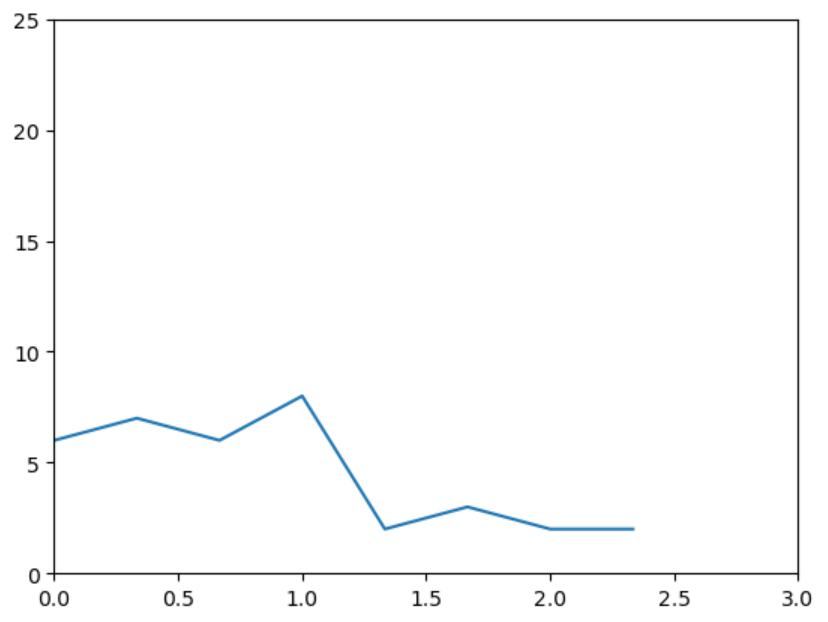
\includegraphics[width=0.4\textheight]{images/Seizure.png}
    \caption{Amount of windows on the vertical axis and smoothed number of spikes on the horizontal axis,This data is from 3 minutes of EEG data in which a seizure occurs.}
    \label{fig:seizure der}
\end{figure}

\begin{figure}
    \centering
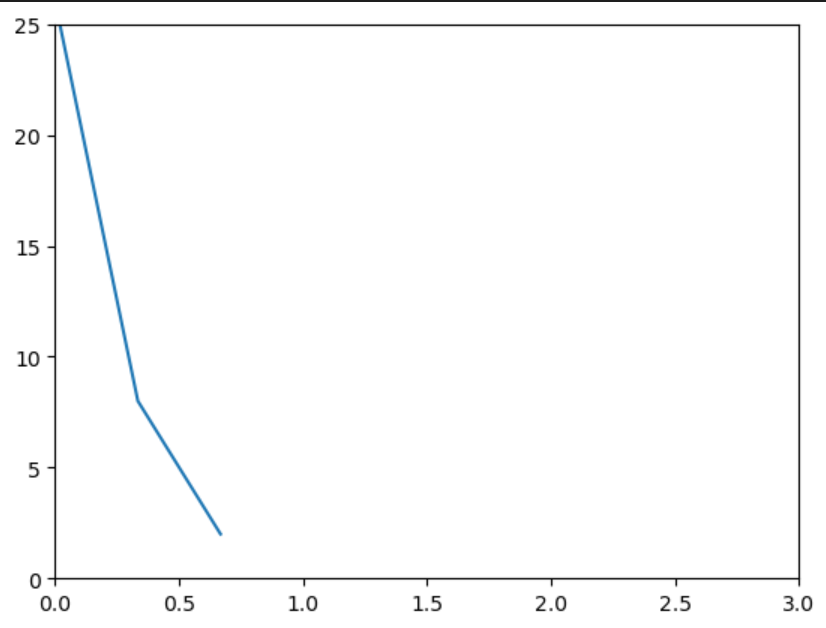
\includegraphics[width=0.4\textheight]{images/540 no seizure.png}
    \caption{Amount of windows on the vertical axis and smoothed number of spikes on the horizontal axis. Data were taken from 3 minutes of the inter-ictal/pre-ictal state.}
    \label{fig:no seizure der}
\end{figure}

%This approach is based on the observation that the distribution of number of spikes mapped against number of windows it occurs in shows a increase in the amount of windows a certain number of spikes occurs in.\\

Since the number of spikes per window has been shown to increase the closer you get to a seizure, it follows that if a graph were made over this behavior, one would be able to correlate a flattening of the resulting curve with a pre-ictal state. Since the closer you get to a seizure the more times a high number of spikes will occur.

%vilket exempel är bäst???????
%Shown below is a example of $N_{smooth}$ mapped against number of windows it occurs in. We can in this graph observe a changing of the flattens of this curve. 

If a derivative is calculated between all data points, and if these derivatives are averaged the resulting value can be used to predict if a seizure is incoming. This threshold will then decide how "flat" the curve has to be on average.

%This criterium can be visualised by the figure below.
%(insert figure of criteria)

In this project, we therefore created an algorithm that works in the following steps:
\begin{itemize}
    \item split each channel into 3 minutes segment. Then split these into 5 seconds windows.
    \item calculate $N_{smooth}$ per window, like the previous method.
    \item sort a list of these values in increasing order. Calculate how many times these occur in the segment. Then calculate the percentage of how many of the total windows a certain $N_{smooth}$ occurs in.
    \begin{align}
        p[i] = \dfrac{\text{number of windows $N_{smooth}$ occurs in}}{\text{total amount of windows in segment}}
    \end{align}
    \item calculate the derivative of each data point of these mapped against each other, according to the formula below.
    \begin{align}
    Der = \sum \dfrac{{p[i+1]-p[i]}}{{N_{smooth}[i+1]-N_{smooth}[i]}}
    \end{align}
    \item Calculate the mean of these derivatives.
    \begin{align}
        MeanDer = \sum \dfrac{Der[i]}{N_{der}}
    \end{align}
    \item if above and below a picked value in two or more channels then a seizure is predicted.
\end{itemize}

%- split each channel into 3 minutes segment. Then split these into 5 seconds windows.

%- calculate $N_{smooth}$ per window, like the previous method.

%- sort a list of these values in increasing order. Calculate how many times these occur in the segment. Then calculate the percentage of how many of the total windows a certain $N_{smooth}$ occurs in.

%\begin{align}
%    p[i] = \dfrac{\text{number of windows $N_{smooth}$ occurs in}}{\text{total amount of windows in segment}}
%\end{align}

%-calculate the derivative of each data point of these mapped against each other, according to the formula below.

%\begin{align}
%    Der = \sum \dfrac{{p[i+1]-p[i]}}{{N_{smooth}[i+1]-N_{smooth}[i]}}
%\end{align}

%-Calculate the mean of these derivatives.

%\begin{align}
%    MeanDer = \sum \dfrac{Der[i]}{N_{der}}
%\end{align}

%- if above and below a picked value in two or more channels then a seizure is predicted.

 


%Since during analysis it was observed that the frequency of these spikes increase the closer you get to the seizure see figure (spike frequency).

%While a promising idea in theory, it turned out to be a dead end, since it did not give any fruitful and meaningfull prediction. Because this behavior do not occur in short enough time spans, similar to the central limit theorem. Due to this realisation this method was discarded in favor of other methods.

%A method was then proposed that calculated the proportion of spike frequency to the number of times in occurred see figure(spike distribution). However this method turned out to be unfruitful, and produced no understandable results, as a consequence the method was discarded.

\subsubsection{Matching filter}
Due to the unpromising nature of these results, the focus was shifted to improving the accuracy of each spike. So a matching filter was constructed to avoid the noisiness and randomness in the signals. This matching filter is meant to be implemented as an alternative to the if statement analysis described in the previous part. This method had two main components, first creating a pattern of a spike and then creating a matching filter to scan the channels for spikes.\\


\subsubsection{Least squares criteria}
An algorithm was created that, according to the aforementioned criteria of what a spike is described, picks out all parts of the signal that goes over the value $100 mV$ and stores it in a list of lists. This list is then cleared of all of the signals that do not adhere to the time criteria of a spike, for each of these the extracted part is then extended to include the surrounding values of the signal to the start and end of when the signal goes over and under $100mV$, so that the resulting extraction is 30 ms. These are then compounded by averaging all of the values in each time step of the signals the resulting signal is regarded as a spike pattern. See the figure(\ref{fig:my_label1}).\\

\begin{figure}
    \centering
    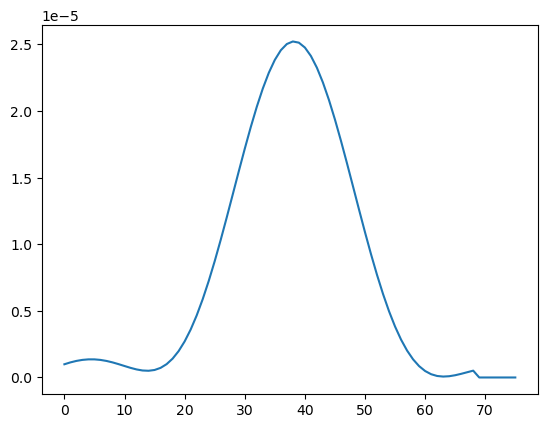
\includegraphics[width=0.4\textheight]{images/Spike_pattern.png}
    \caption{Pattern of a spike}
    \label{fig:my_label1}
\end{figure}

This is then fed to a matching filter that searches for similar patterns in the EEG signal. The matching filter uses a sliding window of the same length as the pattern, and each of these windows is then compared with a least square fit method. This method was described in the paper by Ramachandran et al \cite{MatchingFilter2}. First the squared distance between each point $y$ in the window and the corresponding point $x$ in the pattern.

%insert equation
\begin{align}
    \hat{y}(t) = ax(t) + b
\end{align}
where the parameters of the least square are given by the following equations:

\begin{align}
    a = \frac{\Sigma x(t)y(t) - \Sigma x(t) \Sigma y(t)/N}{\Sigma x{2}(t) - \Sigma x(t) \Sigma x(t)/N}
\end{align}

\begin{align}
    b = \Sigma y(t) - a \Sigma x(t)   
\end{align}

N is the number of samples of the analyzed signals. This formula will give a standard error calculated accordingly:

\begin{align}
    SE = \sqrt{\dfrac{\Sigma(y(t)-\hat{y}(t))^2}{N-1}}
\end{align}

The score for a match is then given by the following:

\begin{align}
    criterion score = \dfrac{a}{SE}
\end{align}

A weakness whit this method is that the $criterion score$ is not a percentage of how much it is similar. It is an exponentially growing index. consider the case when $y(t)$ is the same as $\hat{y}(t)$ in this case $SE$ would be:

\begin{align}
    SE = \sqrt{\dfrac{0}{N-1}} = 0
\end{align}

then the criterion score would tend to infinity:

\begin{align}
    criterionscore = a/0 = \infty
\end{align}

Due to this the criterion score has to be experimentally set and will be hard to have any intuitive meaning. It was in this paper set to be $10217$
%This criterion score was set to be $10217$. This was chosen by tuning.\\
\\

\subsubsection{Pearson correlation coefficient}

Another method for checking for a match was the Pearson correlation coefficient. This was done by calculating the correlation matrix and selecting the element that correlates with the signals. The threshold for this score to clear for a match was set to $0.98$ so as to demand a high degree of similarity to our criteria. For the spike not to be counted twice, an if statement is introduced. This sets the constraint that once a match of $0.98$ is achieved, it will not register another spike until it goes below this value again. 
